\documentclass[a4paper,12pt]{article}

\usepackage[utf8]{inputenc} 
\usepackage{amsmath}
\usepackage[a4paper, margin=0.9in]{geometry} % Adjust the margin here
\usepackage{multirow}
\usepackage{graphicx}
\usepackage{tikz}
\usepackage{wrapfig}
    
\begin{document}


\section*{Question 1}
A particle of mass $m$ moves under the influence of a central force $\vec{F}(r)=\left(-kr+\frac{C}{r^3}\right)\hat{r}$, where $k>0$ and $C>0$ are constants, $r$ is the radial distance from the origin, and $\hat{r}$ is the unit vector in the radial direction.
\begin{itemize}
    \item[(a)] Explain in very simple terms (preferably by using the definition of torque) why the angular momentum of the particle is conserved. --- \textit{0.4 points}
    \item[(b)] Find the effective potential of the particle is given as $V(r)=U(r)+\frac{l^2}{2mr^2}$, where $U(r)$ is the potential of the particle and $l$ is the angular momentum. --- \textit{0.4 points}
    \item[(c)] Find the equilibrium point(s) of the particle. What values can $C$ take for an equilibrium point to exist?--- \textit{0.2 points} 
\end{itemize}

\section*{Question 2}
Consider two identical pendulums as shown in the figure, each consisting of a mass $m$ attached to a string of length $L$ suspended from the same point. The pendulums are initially at rest. The pendulum $A$ is released from a height $h$ relative to $B$, while the pendulum $B$ is initially stationary.
\begin{figure}[h]
    \centering
    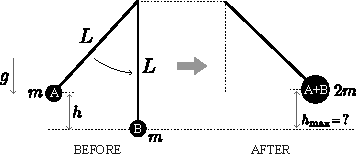
\includegraphics[width=0.55\textwidth]{figures/q2.pdf}
\end{figure}
\begin{itemize}
    \item [(a)] Determine the velocity of the pendulum $A$ just before it collides with the pendulum $B$. ~-- \textit{0.4 points}
    \item [(b)] After the collision, the two pendulums stick together and swing as one system. Calculate the maximum height reached by the combined system after the collision. -- \textit{0.6 points}
\end{itemize}

\section*{Question 3}
\begin{figure}[h]
    \centering
    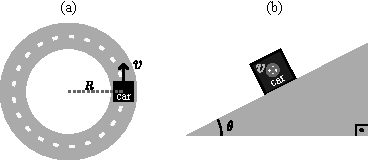
\includegraphics[width=0.65\textwidth]{figures/q3.pdf}
    \label{fig:q4}
\end{figure}
\noindent
A car of mass $m$ is moving at a speed $v$ around a curve with a radius $R$. The coefficient of static friction between the tires and the road is $\mu_s$, and the gravitational acceleration is $g$.

\begin{itemize}
    \item [(a)] Determine the maximum speed $v_{\text{max}}$ at which the car can navigate the curve safely to avoid slippage as shown in Figure (a). --- \textit{0.7 points}
    
    \item [(b)] If the road is banked as shown in Figure (b) at an angle $\theta$ with respect to the horizontal, find the maximum speed for which the car can take the curved path safely \underline{without depending on friction}. --- \textit{0.3 points}
\end{itemize}
\underline{Note}: All the other other external forces, such as air resistance, are negligible.

\section*{Question 4}
\begin{figure}[h]
    \centering
    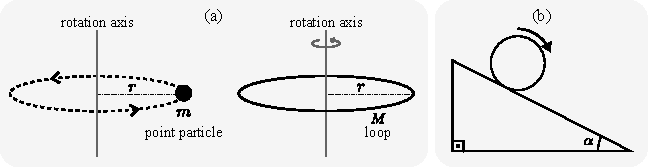
\includegraphics[width=0.95\textwidth]{figures/q4.pdf}
    \label{fig:q4}
\end{figure}

    \begin{itemize}
    \item[(a)] Given that the rotational inertia of a point particle as shown in the Figure (a) is $mr^2$, explain why the rotational inertia of a uniform loop would be $Mr^2$? --- \textit{0.2 points}
    \item[(b)] Calculate the acceleration of a uniform loop as it \underline{rolls without sliding} on a rough inclined plane inclined at an angle $\alpha$ to the horizontal as shown in Figure (b), in a uniform gravitational field of magnitude $g$. --- \textit{0.8 points}
\end{itemize}




\end{document}
